\documentclass[czech,bachelor]{../../shared/diploma}

\usepackage[autostyle=true,czech=quotes]{csquotes} % korektni sazba uvozovek, podpora pro balik biblatex
\usepackage[backend=biber, style=iso-numeric, alldates=iso]{biblatex} % bibliografie
\usepackage{dcolumn} % sloupce tabulky s ciselnymi hodnotami
\usepackage{subfig} % makra pro "podobrazky" a "podtabulky"

\usepackage{float} % lepsi umistovani obrazku (H)

% Pozadovane vstupy pro generovani titulnich stran.
\ThesisAuthor{Miroslav Osoba}
\ThesisSupervisor{doc. Ing. Radoslav Fasuga, Ph.D.}

\CzechThesisTitle{Tvorba uživatelského prostředí výpravné evoluční hry}
\EnglishThesisTitle{Creation of the User Environment for the Narrative Evolution Game}

\SubmissionYear{2024}

\ThesisAssignmentFileName{../specification.pdf}

\Acknowledgement{TODO Acknowledgement}

\CzechAbstract{TODO Cz Abstract}
\CzechKeywords{hybridní desková hra; uživatelské prostředí}

\EnglishAbstract{TODO En Abstract}
\EnglishKeywords{hybrid board game; user environment}

\addbibresource{resources/sauce.bib}

% Novy druh tabulkoveho sloupce, ve kterem jsou cisla zarovnana podle desetinne carky
\newcolumntype{d}[1]{D{,}{,}{#1}}

% Uprava hloubky obsahu - pozdeji smazat !
\setcounter{tocdepth}{2}


% Zacatek dokumentu
\begin{document}

% Titulni strany
\MakeTitlePages

% Seznam obrazku
% \listoffigures
% \clearpage

% Seznam tabulek
% \listoftables
% \clearpage

% Text zaverecne prace.
\chapter{Úvod}

Welcome to hell. This is the introduction chapter.

\chapter{Hybridní hry}
Hybridní hry kombinují jak prvky fyzické, tak digitální. Jedná se o~hry, které mají jakékoliv napojení na technologii, ať už je to elektronické bankovnictví ve hře \textit{Monopoly Super Electronic Banking} či mobilní aplikace \textit{Pokémon GO}, která uživatele pomocí map navádí k~navštívení památek a~zajímavých míst. Podobná spojení vyústí ve zcela nové herní zážitky, které si hráči mohou vyzkoušet. \cite{hybrid_board_games_design}

\section{Vývoj hybridních her}
První hybridní hry se začaly formovat již na začátku 20. století, kdy se začaly objevovat první hry s~elektronickými prvky. Tyto hry byly většinou jednoduché elektrické obvody, které hráč propojoval pro různé efekty. V~průběhu času se tyto hry stávaly složitějšími a~začaly se objevovat takové, které využívaly počítačové technologie. Hybridní hry mohou být kategorizovány do několika skupin, které se liší podle toho, jakým způsobem technologie využívají. \cite{history_of_hybrid_games}

\subsection{Stolní hry s~vlastním zařízením}
Mezi takovéto hry patří již výše zmíněné \textit{Monopoly Super Electronic Banking}, které obsahují elektronické bankovnictví, nebo známá hra \textit{Operation}, ve které se hráči nesmí dotknout kovových částí na hrací desce, jinak se rozezní siréna. 

Tato kategorie hybridních her je rozhodně nejstarší. První hrou využívající elektrického proudu, a~tudíž zařazenou do hybridních her, je hra \textit{Electra} (původním názvem \textit{Lichtra}), kterou můžeme vidět na Obrázku \ref{fig:electra}. Jedná se o~jednoduchou kvízovou hru, která vyšla už v~roce 1910 v~Německu a~byla vytvořena společností \textit{Sala Games}. Hra obsahovala jednoduchý elektrický obvod, který se uzavřel, pokud hráč odpověděl správně. Po ní následovala dlouhá éra her, jejichž elektronika také spočívala pouze v~propojení jednoho či několika málo obvodů. \cite{history_of_hybrid_games, boardgames_with_apps}

\begin{figure}[H]
    \centering
    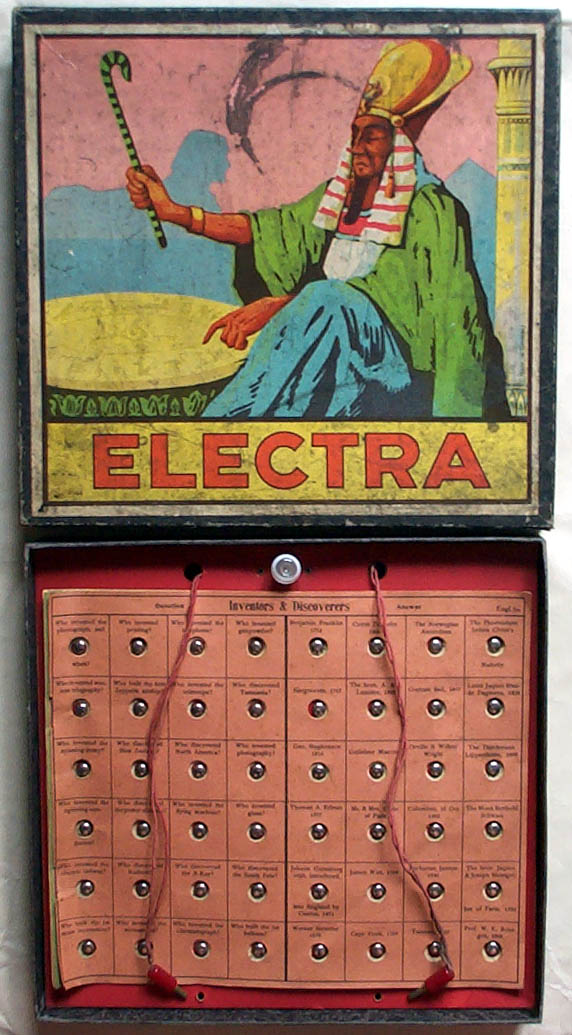
\includegraphics[width=0.3\textwidth]{resources/figures/electra.jpg}
    \caption{Hra \textit{Electra}, první hybridní hra \cite{history_of_hybrid_games}}
    \label{fig:electra}
\end{figure}

Další zmínku ve vývoji her v~této kategorii si zasloužila hra \textit{Voice of the Mummy}, která vyšla v~roce 1971. Ta měla v~herním plánu zabudovaný přehrávač, který měl simulovat hlas mumie, která při přechodu přes určitá herní pole hráčům určovala další postup. \cite{voice_of_the_mummy}

První hrou, která ve svém designu používala počítačové zařízení, byla francouzská hra \textit{Simulateur JR10}, která vyšla v~roce 1972. Jednalo se o~bitevní hru, ve které hráči ovládali různé bojové jednotky. Při střetu se do počítače vložil děrný štítek s~odpovídajícími jednotkami a~počítač podle naprogramovaných kritérií náhodně určil výsledek střetu. \cite{simulateur_jr10}

\subsection{Stolní hry s~vlastní aplikací}
V~roce 1972 vyšla herní konzole \textit{Magnavox Odyssey}, která je uznávaná jako první domácí herní konzole na světě. Zároveň s~ní vyšlo i~několik her, které kombinovaly fyzickou hrací desku s~počítačovým programem. Celé UI této konzole zahrnovalo pouze několik svítících bodů na obrazovce, proto byl ke každé hře přiložen lehce průsvitný plán s~potiskem, který se na obrazovku přichytil. Součástí většiny her byly i~fyzické komponenty, které měly hráčům sloužit k~přirozenějšímu pozvolnému přechodu ze stolních her na hry digitální. \cite{magnavox_odyssey} Jednou z~her vytvořenou pro tuto konzoli byla hra \textit{Invasion}, jejíž fyzická složka zahrnovala kostky, sadu karet, sadu tokenů a~hrací desku. Samotný program byl pak určen k~soubojům mezi hráči. Tyto komponenty můžeme vidět na Obrázku \ref{fig:invasion} \cite{invasion,invasion_gameplay}

\begin{figure}[H]
    \centering
    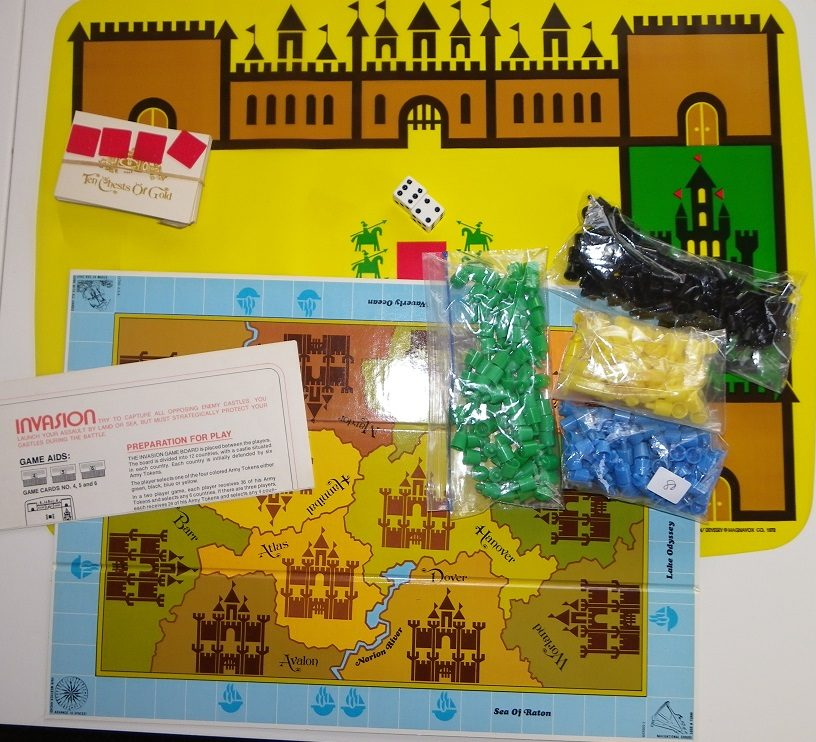
\includegraphics[width=0.45\textwidth]{resources/figures/invasion.jpg}
    \caption{Fyzické komponenty a~nalepovací plán hry \textit{Invasion} \cite{invasion}}
    \label{fig:invasion}
\end{figure}

V~roce 1983 vyšlo hned několik her, které kombinovaly fyzickou hrací desku s~digitálním prostředím. Jednou z~nich byla společností \textit{Epyx} vydaná hra \textit{Oil Barons}. Jednalo se o~počítačovou hru, která byla určena pro zařízení \textit{DOS}, \textit{Apple II} a~\textit{Commodore 64}. Její součástí byla fyzická hrací deska a~několik herních tokenů. Samotný program měl za úkol simulovat náhodné výsledky a~udržovat stav hry. UI této hry bylo jednoduché a~odpovídalo své době, jak lze vidět na Obrázku \ref{fig:oil_barons}. \cite{oil_barons}

\begin{figure}[H]
    \centering
    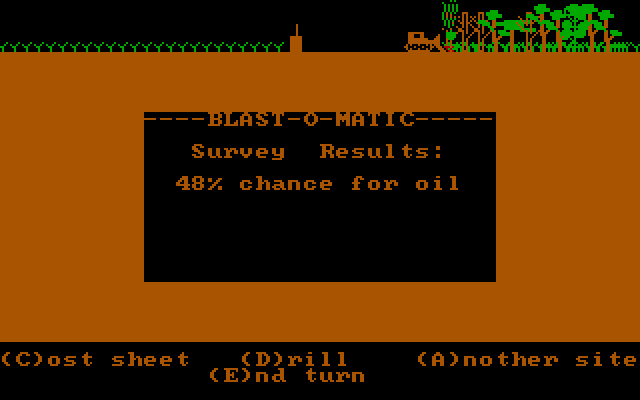
\includegraphics[width=0.45\textwidth]{resources/figures/oil_barons.png}
    \caption{Příklad GUI hry \textit{Oil Barons} \cite{oil_barons}}
    \label{fig:oil_barons}
\end{figure}

Další významný vývoj této kategorie hybridních her se ubíral nejčastěji k~mobilním aplikacím a~takzvaným companion apps (podpůrným aplikacím). Tyto aplikace slouží k~různým účelům, jako je například výběr či správa herních prvků nebo vyprávění příběhu. Většina těchto aplikací je oficiální součástí dané hry a~bez jejího použití není možné ji odehrát. Mezi ně patří například hra \textit{Na vlnách neznáma} (původním názvem \textit{Forgotten Waters}), která využívá aplikaci k~vyprávění příběhu, správě nepřátel a~k~výběru dějové linky.

\subsection{Hry s~rozšířenou realitou}
Nejmladší kategorií hybridních her jsou hry s~rozšířenou realitou (augmented reality, neboli AR). Tyto hry využívají technologie, které umožňují hráčům interagovat s~digitálními prvky ve skutečném světě. První takovou hrou byla \textit{AR Quake}, která byla vytvořena v~roce 2000. Aby si ji hráč mohl vyzkoušet, musel mít nasazený speciální batoh s~počítačem, který pomocí gyroskopů určoval jeho polohu a~promítal obraz digitálního světa přes speciální brýle. Hra byla vytvořena jako experiment, který měl ukázat možnosti AR technologií. \cite{ar_history}

Největší rozvoj v~popularitě AR her nastal až s~vydáním aplikace \textit{Pokémon GO} v~roce 2016. Tato hra využívala GPS a~kameru mobilního telefonu k~tomu, aby hráči ve skutečném světě mohli hledat a~chytat virtuální postavičky. Hra byla velice populární a~stala se tak první AR hrou, která se dostala do povědomí široké veřejnosti.

\section{Vybrané hybridní hry}
Následující hry jsem vybral jako příklady a~inspiraci pro tuto práci. Jedná se o~stolní hry, které nějakým způsobem využívají právě internetových aplikací pro umocnění herního zážitku, organizaci hry či správu herních mechanismů.

\subsection{Na vlnách neznáma}
První z~těchto her je \textit{Na vlnách neznáma}, vydaná v~roce 2020 společností \textit{Plaid Hat Games}. Jedná se o~výpravnou RPG hru, ve které se hráči ujímají rolí pirátů a~společně čelí dobrodružstvím a~nástrahám, jež rozmanitý příběh této hry nabízí. Hra samotná využívá oficiální internetovou aplikaci \cite{forgotten_waters_app}, která slouží k~vyprávění herního děje pomocí namluvených scén a~k~zaznamenávání hráčských rozhodnutí, na kterých závisí dynamický rozvoj příběhu této hry. Aplikace dále udává životy a~statistiky nepřátel, slouží k~výběru kampaně (dějové linky) a~v~neposlední řadě přispívá k~zážitku hráčů pomocí namluvených scén.

Fyzické komponenty hry obsahují herní plán s~hexagonálními políčky a~s~tokeny lokací, které si hráči rozestaví podle pokynů aplikace. Dále obsahuje kartonové figurky, osobní deníky postav, knihu lokací, balíček karet a~sadu kostek. Kartonové figurky s~potiskem v~kombinaci s~osobními deníky, do kterých si hráči zapisují informace, představují postavy. Zároveň se ve hře nachází několik ukazatelů a~počítadel, jež se využívají v~různých aspektech hry. V~knize lokací lze najít popisy míst, které mohou hráči ve hře navštívit, a~zároveň možnosti, jež se jim v~těchto lokacích nabízejí. Karty v~balíčku představují poklady a~úryvky příběhu. Oba tyto druhy přináší hráči buďto pozitivní nebo negativní efekty, které ovlivňují jeho postavu. Sada kostek se využívá k~určování výsledků různých akcí, jež hráči mohou provést.

\subsection{Gloomhaven}
Druhou hrou, kterou bych chtěl uvést, je \textit{Gloomhaven}. Tato hra byla vydána v~roce 2017 společností \textit{Cephalofair Games}. Jde o~kooperativní fantasy hru, ve které se hráči vcítí do role dobrodruhů, jenž se snaží přežít v~nehostinném světě, plnit různé úkoly a~odkrývat příběh, který před nimi leží. Hra je ve stylu dungeon crawl, což znamená, že hlavní náplní hry je postup z~lokace do lokace, kde hráče čekají úkoly a~boj s~nepřáteli. Původně je hra koncipována jako čistě stolní hra, ale kvůli velkému množství fyzických komponent (Obrázek \ref{fig:gloomhaven_contents}), které hra obsahuje, začaly vznikat aplikace, jež mají za úkol organizaci hry usnadnit. Jednou z~nich byla aplikace \textit{Gloomhaven Helper} \cite{gloomhaven_helper}, která se na čas stala i~oficiální aplikací pro tuto hru, avšak kvůli licenčním problémům byla zrušena. Po jejím stažení z trhu vzniklo několik nástupců. Jedním z~nich je \textit{Gloomhaven Secretariat} \cite{gloomhaven_secretariat}, který slouží k~organizaci hry, správě nepřátel i~postav. Také umožňuje hráčům zaznamenávat své postupy v~příběhu, výsledky bitev a~další herní prvky.

\begin{figure}[H]
    \centering
    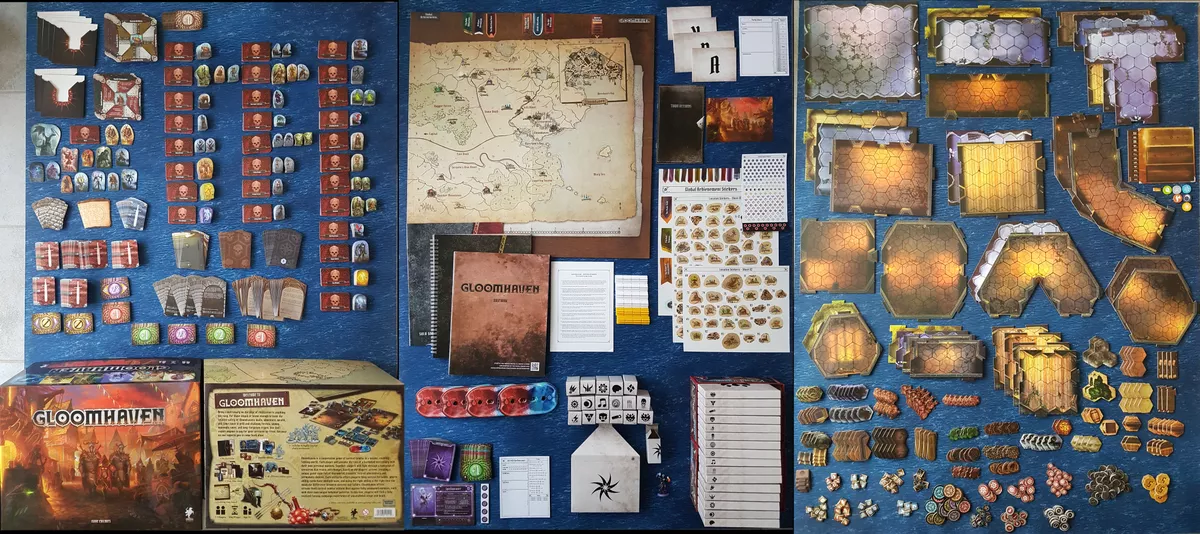
\includegraphics[width=0.9\textwidth]{resources/figures/gloomhaven.png}
    \caption{Fyzické komponenty deskové hry \textit{Gloomhaven} \cite{gloomhaven}}
    \label{fig:gloomhaven_contents}
\end{figure}

Fyzická součást hry obsahuje mapu světa, na kterou hráči postupně přilepují nálepky odemčených lokací a~svých úspěchů. Hra obsahuje díly lokací, což jsou části hrací desky, které lze složit k~sobě. Tyto části jsou potištěny hexagonovou sítí, která slouží jako políčka pro hráčské figurky. Dále se zde nachází kniha lokací, která popisuje příběh a~udává rozložení a~díly potřebné pro složení jednotlivých lokací. Každý typ nepřítele má svou kartu statistik a~vlastní balíček karet, které určují jeho chování a~možné akce. Pro všechny nepřátele existuje jeden společný balíček modifikátorů (karet, které namísto kostek slouží k~vytváření nahodilých výsledků). Podobně má každá postava také svou sadu karet akcí a~velkou kartu statistik, zároveň má však každý hráč vlastní balíček modifikátorů a~počítadlo životů. Figurky postav jsou vyrobeny z~plastu a~jsou velice detailní. Kartonové figurky s~plastovými stojánky představují nepřátele. Dále hra obsahuje velké množství kartiček předmětů, které hráči mohou používat, tokeny peněz, poškození a~efektů.
\chapter{Uživatelské rozhraní}

\section{Stručná historie GUI}
Počátek grafických rozhraní se datuje do osmdesátých let minulého století, kdy firma Xerox vyvinula počítač Alto. Jednalo se o první počítač, jehož rozhraní se skládalo z oken, ikon a používalo myš k ovládání. Toto grafické rozhraní pak posloužilo jako odrazový můstek a základ dalším projektům. Jeden z nich byl například Apple Macintosh, který grafické uživatelské rozhraní popularizoval. Dále přišel operační systém Windows, který GUI posunul ještě dál mezi mainstreamové uživatele. GUI se postupem let vyvíjelo společně s novými technologiemi a nyní je neoddělitelnou součástí téměř všech počítačových systémů.

\section{Zásady vývoje webového GUI}
Následující zásady jsou základem přívětivého UI, ve kterém se dokáže uživateů snadno orientovat a které je příjemné na pohled. Vychází z praktických zkušeností grafiků i psychologických poznatků. 

% \subsection{Vzhled}
\subsection{Obecné zásady}
Následující text se věnuje nejzákladnějším principům, které by mělo uživatelské rozhraní splňovat.\cite{principles_of_design}

\subsubsection*{Kontrast}
Kontrast je jedním z nejdůležitějších prvků designu. Zajišťuje, že text a další prvky jsou čitelné a viditelné. Je důležitý pro umocnění dojmu a pro zvýraznění důležitých prvků.

\subsubsection*{Balanc}
Všechny prvky na stránce mají pomyslou váhu, která je dána jejich velikostí, barvou, kontrastem a dalšími faktory. Zajišťuje, že tyto prvky jsou rozloženy tak, aby stránka působila vyváženě a přehledně.

\subsubsection*{Důraz}
Důraz slouží pro zvýraznění důležitých prvků a k pomyslnénu ukrytí těch méně podstatných. Můžeme tak ovládat výraznost jistých informací a zároveň usměrňovat pozornost uživatele.

\subsubsection*{Proporce}
Správně určené proporce podporují výše zmíněný balanc. Pomáhají uživateli orientovat se na stránce a zároveň zajišťují, že stránka působí přehledně a esteticky.

\subsubsection*{Hierarchie}
Hierarchie je v designu klíčová, zejména pokud jde o zdůraznění důležitých prvků. Tento princip je často demonstrován prostřednictvím titulů a nadpisů. Titul stránky by měl okamžitě vyniknout jako nejdůležitější prvek, zatímco nadpisy by měly být formátovány tak, aby naznačovaly svůj význam ve vztahu k sobě navzájem a k obsahu, který uvádějí.

\subsubsection*{Opakování}
Opakování je účinným nástrojem pro zdůraznění a sjednocení myšlenek v rámci designu. Lze ho dosáhnout konzistentním použitím barev, písem, tvarů nebo jiných prvků designu. Konzistentní formátování pomáhá sjednotit prvky na celé stránce.

\subsubsection*{Rytmus}
Slovem rytmus je myšlen styl, jakým jsou prvky (ať už mezery, barvy, velikosti, atd.) na stránce uspořádány a v jakém pořadí použity. Některé rytmické vzory mohou vzbuzovat pocit uspořádanosti a přehlednosti, zatímco jiné mohou působit chaoticky.

\subsubsection*{Vzor}
V uživateli vzory vyvolávají pocit předvídatelnosti a pohodlí. Může se jednat například o rozložení stránky, které se běžně používá, nebo o způsob zadávání dat, který je uživatelům známý.

\subsubsection*{Volný prostor}
Volný prostor (white space) je prázdný prostor mezi prvky na stránce, který pomáhá zvýraznit důležité prvky a zároveň zajišťuje, že stránka není přeplněná.

\subsubsection*{Pohyb zraku po stránce}
Tohoto principu lze dosáhnout dodržením výše zmíněných prvků. Jde o kombinaci všech předešlých principů a jejich aplikaci tak, aby uživatel mohl snadno a pohodlně stránku použít.

\subsubsection*{Rozmanitost}
Na rozdíl od předešlých bodů, rozmanitost nenapomáhá orientaci na stránce, ale zajišťuje, aby byla pro uživatele zajímavá.

\subsubsection*{Spojitost}
Spojitost zajišťuje, že všechny prvky na stránce působí jako celek. Většinou se jedná o opakování barev, či používání minimálního množství fontů.

% \begin{itemize}
%     \item \textbf{Kontrast}: Zajišťuje, že text a další prvky jsou čitelné a viditelné.
%     \item \textbf{Balanc}: Udržuje vyváženost prvků na stránce.
%     \item \textbf{Důraz}: Zvýrazňuje důležité prvky a pomáhá usměrňovat pozornost uživatele.
%     \item \textbf{Proporce}: Podporují balanc a pomáhají uživateli orientovat se na stránce.
%     \item \textbf{Hierarchie}: Důležitá pro zdůraznění prvků, zvláště titulů a nadpisů.
%     \item \textbf{Opakování}: Slouží k sjednocení myšlenek v rámci designu.
%     \item \textbf{Rytmus}: Určuje uspořádání prvků na stránce, což může vyvolat pocit přehlednosti.
%     \item \textbf{Vzor}: Vybuzuje pocit předvídatelnosti a pohodlí.
%     \item \textbf{Volný prostor}: Pomáhá zvýraznit důležité prvky a udržuje stránku přehlednou.
%     \item \textbf{Pohyb zraku po stránce}: Pořadí v jakém si uživatel prvků všimne. Zajišťuje to kombinace předešlých principů.
%     \item \textbf{Rozmanitost}: Zajišťuje, aby stránka byla zajímavá pro uživatele.
%     \item \textbf{Spojitost}: Zajišťuje, že všechny prvky působí jako celek.
% \end{itemize}

\subsection{Teorie barev}
Výběr barev je nedílnou součástí vývoje každého GUI. Teorie barev se zabývá vztahy mezi barvami a jejich významem. Poznáním těchto nuancí může vývojář využít barvy k ovlivnění uživatelova vnímání své aplikace. Různé barvy mohou budit různý psychologický a emocioální význam. Teorie barev poskytuje základní pravidla a směrnice pro efektivní použití barev v designu, aby se dosáhlo esteticky příjemného výsledku a vyvolalo se požadované emoční nebo vizuální působení. Teorie barev také udává, že existuje několik kategorií základních barev:
\begin{itemize}
    \item \textbf{Primární barvy}: Červená, modrá a žlutá. Tyto barvy nelze vytvořit kombinací jiných barev.
    \item \textbf{Sekundární barvy}: Zelená, fialová a oranžová. Tyto barvy vzniknou smícháním dvou primárních barev.
    \item \textbf{Terciární barvy}: Těchto šest barev vznikne smícháním primárních a sekundárních barvev. Patří sem například růžová, tyrkysová, či žlutozelená.
\end{itemize}

Těchto dvanáct barev samozřejmě není jedinými barvami, které lze zejména v počítačové grafice použít. Díky tomu se začalo v grafice používat takzvaný color wheel (barevný kruh).\cite{color_theory_design}

\subsubsection{Color wheel}
Barevný kruh se často používá díky jeho intuitivnímu rozložení barev. Obsahuje všechny barvy, které lze vytvořit smícháním tří primárních barev a díky přidání černé, či bílé barvy umožňuje i úpravu jejich odstínů. Existuje několik způsobů, jak za pomoci tohoto kruhu vybrat:
\begin{itemize}
    \item \textbf{Komplementární}: Barvy, které jsou na opačných stranách kruhu. Při jejich kombinaci vzniká kontrastní efekt.
    \item \textbf{Monochromatické}: Tyto barvy je sada odstínů jedné barvy. Vytváří harmonický efekt.
    \item \textbf{Analogické}: Barvy, které jsou vedle sebe na kruhu. Vytváří přirozený a pohodlný efekt, ale je vhodné vybrat jednu z barev jako hlavní a zbytek používat pouze jako akcenty.
    \item \textbf{Triadické}: Kombinace tří barev, které na kruhu tvoří rovnostranný trojúhelník. Podobně jako způsob komplementární, také vytváří kontrastní efekt.
    \item \textbf{Tetradické}: Čtyři barvy, které jsou od sebe na kruhu položeny stejně daleko. Vytváří podobný efekt jako triadický způsob, ale je těžší je správně kombinovat.
\end{itemize}\cite{color_wheel}

% \subsection{Použitelnost}

\section{GUI ve vybraných hybridních hrách}

\subsection{Na vlnách neznáma}
Aplikace pro hru Na vlnách neznáma je primárně zamýšlená pro mobilní zařízení, čemuž odpovídá její design. Jedná se o responzivní jednostránkovou aplikaci. Samotná stránka obsahuje základní nastavení přístupnosti a jazyka, informace o aplikaci samotné a především možnost hru spustit. Po spuštění zůstane na stránce pouze jednoduchý vstup pro číslo, které představuje záznam, jenž má aplikace zobrazit. Vždy je možné otevřít historii předešlých záznamů, náhled mapy a časovač. Při načtení záznamu se zobrazí možnosti, které nabízí, a stránka spustí naraci příběhu, který je v něm obsažen. Samotná aplikace je velmi jednoduchá a přímočará, takže představuje ideální doprovod k samotné hře. Věnuje také velkou pozornost přívětivé grafice, což také napomáhá imerzi.


\subsection{Gloomhaven}
Gloomhaven Secretariat je jedna z aplikací pro hru Gloomhaven, která se stará o její největší část, a to souboje. Opět se jedná o jednostránkovou webovou aplikaci. Stránka je primárně určena pro desktop, či jiná zařízení s velkou obrazovkou. Je sice použitelná i na mobilních zařízeních, ale jedná se pouze o zmenšenou verzi klasické stránky bez dalších úprav. To znamená, že některá tlačítka jsou příliš malá pro pohodlné používání. Obsah se také zdá být poměrné jednoduchý, avšak už není tak intuitivní, jako u předešlého příkladu. Po otevření stránky se zobrazí spousta informací a novému uživateli se tak může snadno stát, že se v nich ztratí. Po spuštění aplikace hráče mimo jiné vyzve k výběru příběhové linie, kterou chtějí začít a následně k přidání postav. Stránka pak nabízí spoustu možností, které jsou uživateli k dispozici, ale k žádné z nich nedodá hlubší vysvětlení. Stránka potřebuje neustálé vstupy, aby plnila svou funkci, ty jsou však také někdy neintuitivní a jejich zadávání zdlouhavé.

\section{Volba technologií pro vývoj GUI}
Zprvopočátku jsem vytvořil prototyp GUI v čistém HTML a CSS, abych věděl, jak bude samotný produkt zhruba vypadat. Poté jsem svou pozornost obrátil na výběr technologií, které budu pro vývoj GUI používat. Hlavními kandidáty byly frameworky React, Angular a Svelte.

\subsection{Frameworky}

\subsubsection{React}
React je jednou z nejpopulárnějších moderních platforem pro tvorbu webových aplikací. Je to open-source JavaScript knihovna vyvinutá a udržovaná společností Meta (bývalý Facebook). Používá deklarativní programovací paradigma, což znamená, že vývojář specifikuje, jak by měl výsledek vypadat, bez toho, aby musel explicitně popsat, jak daného výsledku dosáhnout. Zároveň je založen na komponentovém přístupu -- celý kód je rozdělen do menších celků zvaných komponenty, což je kombinace JS a HTML, které jsou modulární a znovupoužitelné. Díky jeho schopnosti aktualizovat jednotlivé komponenty se nejčastěji používá pro vývoj jednostránkových webových aplikací. React je známý svou komunitou a ekosystémem, který je kolem něj postavený. Díky tomu je možné najít spoustu předpřipravených komponent a knihoven, které urychlí vývoj aplikace. Zároveň má však poměrně strmou křivku učení, což z něj dělá nepřívětivou volbu pro začátečníky.

React využívá virtuální DOM, který zajišťuje rychlejší a efektivnější vykreslování změn. Při změně v komponentě se nevykreslí celá stránka, ale pouze upravená část. Tím se značně zrychlí vykreslování a zároveň sníží nároky na výkon.\cite{react, what_react_is_and_why_it_matters,angular_vs_react}

\subsubsection{Angular}
Angular je další z vysoce populárních frameworků pro vývoj UI. Opět se jedná o open-source platformu, nyní však vyvinutou a udržovanou společností Google. Angular je založen na jazyce TypeScript a stejně jako React využívá komponentového přístupu a deklarativního programovacího paradigmatu. Jeho převážný význam spočívá ve vytváření rozsáhlých dynamických webových aplikací. Na rozdíl od Reactu se jedná o plněhodnotný framework, který používá reálný DOM. Samotný framework je robustní a bezpečný, což z něj dělá ideální volbu pro vývoj aplikací, které pracují s citlivými daty. Na druhou stranu je však poměrně složitý a náročný na výkon, což je pro menší aplikace nevhodné.\cite{what_is_angular,angular_vs_react}

\subsubsection{Svelte}
Svelte je moderní framework pro tvorbu webových aplikací. Jedná se o open-source software vyvinutý Richem Harrisem. Svelte se od ostatních frameworků liší tím, že se jeho kód při buildu převede na čistý optimalizovaný JavaScript. Tím se výsledná aplikace značně zrychlí a zároveň se sníží nároky na výkon na straně uživatele. Svelte také nabízí velmi jednoduchý a přívětivý způsob psaní kódu, který vývoj aplikace urychlí. Dokáže také pracovat s TypeScript soubory bez nutnosti jejich předešlé kompilace, což výsledný kód dělá mnohem bezpečnějším a přehlednějším.\cite{svelte_and_why_you_should_consider_it,svelte}

\subsubsection{Srovnání}
Vzhledem k tomu, že projekt obnáší vytvořiení GUI pro hybridní stolní hru, která nebude nijak extrémně rozsáhlá, a zároveň bude potřebovat co největší rychlost a efektivitu, byl nakoinec vybrán framework Svelte. Ten nabízí všechny potřebné funkce a zároveň je velmi rychlý a efektivní. Jeho jednoduchost by také měla přispět k rychlejšímu vývoji bez dalších větších problémů.

\subsection{Další technologie}
Dále jsem se rozhodl používat CSS knihovny, které dokáží ušetřit práci s designem a responzivitou a zároveň zrychlí vývoj aplikace. Jako hlavní kandidáti se ukázaly Bootstrap a Tailwind CSS. Bootstrap je velmi populární knihovna, která nabízí spoustu předpřipravených komponent a stylů. Tailwind CSS je naopak známý svou flexibilitou a možnostmi přizpůsobení.
***V plánu rozepsat.***

% Seznam literatury
\printbibliography[title={Literatura}, heading=bibintoc]

\end{document}
